\documentclass[10pt,a4paper]{article}
\usepackage{graphicx}
\usepackage[margin=0.5in]{geometry}

\begin{document}
\title{Airport Kernel Driver}
\maketitle

\begin{abstract}
This document describes airport implementation as a kernel driver. Airport has takeoff and landing strips and a hangar. Planes in the air will be implemented as processes in the user land. For plane to land it should be able to successfully execute write method of landing strip device. For plane to take off it needs to successfully execute read method of takeof strip device.

\tableofcontents

\section{Components}
\subsection{Monitor}
Monitor is a separate process that memmap internal hangar memory. It outputs formatted contents of the memory to stdout.

\subsection{Device Airport Hangar}
Airport Hangar accepts planes from the landing strip, and once it has enough passengers for a single plane it is ready to dispatch one plane to a takeoff strip

Airport hangar can have variable number of planes to keep up, to a set number. Airport hangar internal implementation is based on kfifo, that means planes are leaving the hangar in the order they arrived.
Each airplane has a passenger capacity and as soon as there is enough passengers plane is ready for takeoff.

Passengers are delivered to the hangar via kthread that wakes up randomly and generates random number of passengers each time;

Passengers are taken away by another kthread that wakes up randomly and takes away random number of passengers.

\subsection{Device Airport Land Strip}
Airport Land Strip Device accepts planes from the user land. Land strip has a capacity of planes it can handle at the same time. If maximum number of planes are already using land strip then plane is denied access. Plane leaves land strip as soon as there is available space in Airport Hangar.

\subsection{Device Takeoff Strip}
Airport Takeoff Strip device accepts planes from the Airport Hangar device. It has a capacity of maximum planes it can handle.

\subsection{Plane}
Plane is implemented as a user land process. Each plane has it's ID and passenger capacity.
Passenger capacity is chosen randomly but never exceed 300 passengers. Once in the Airport hangar plane does not leave until it has full capacity

\begin{enumerate}
\item In order to land plane needs to call write on Landing Strip device, passing in its ID and capacity.
\item In order to take off plane need to call read on Takeoff Strip device. Once read executed successfully plane process exits.
\end{enumerate}

\subsection{Plane Dispatcher}
Dispatcher generates planes, i.e. user land processes. Planes are generated at random intervals, not exceeding 2 seconds

\section{Diagram}
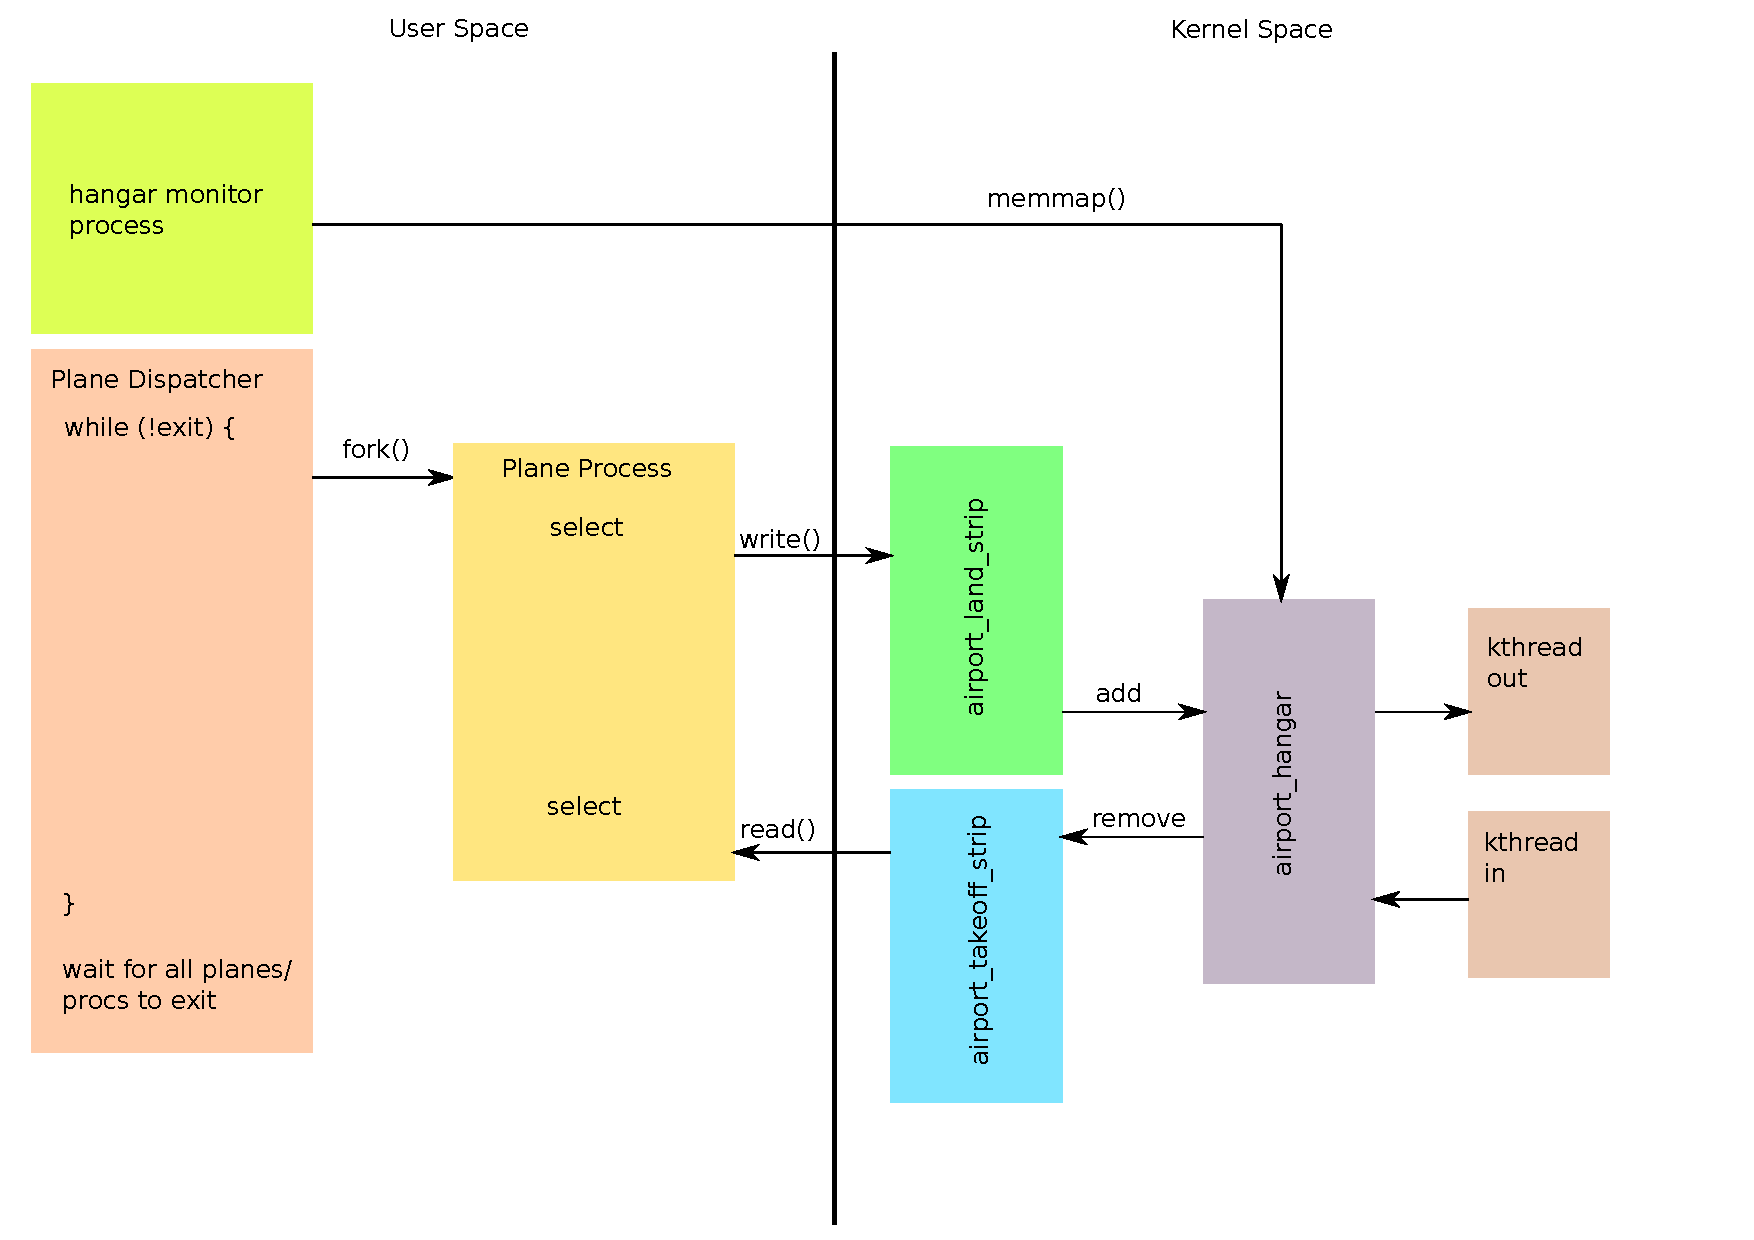
\includegraphics[width=\textwidth]{concept_diag.pdf}


\end{abstract}
\end{document}